\documentclass{article}

\usepackage{graphicx}
\usepackage[margin=1in]{geometry}
\usepackage{listings}
\lstset{
basicstyle=\small\ttfamily,
columns=flexible,
breaklines=true
}
\usepackage{hyperref}
\usepackage{caption, subcaption}
\captionsetup[subfigure]{justification=centering}

\begin{document}

\begin{table}

\caption{Values of the High Cost County Dummy Variable Across Data Sets}

\begin{center}
% latex table generated in R 4.3.2 by xtable 1.8-4 package
% Tue Aug 27 18:28:04 2024
\begin{tabular}{lccc}
  \hline
Sample & NaN & 0 & 1 \\ 
  \hline
OK (2022) &   0 & 1282735 & 524582 \\ 
  LPW (2023) Table 5 &   0 & 2552216 & 1181257 \\ 
  LPW (2023) Table 7 & 32030 & 2545637 & 2599249 \\ 
   \hline
\end{tabular}


\end{center}

\end{table}

\begin{table}

    \caption{LPW Table 7 -- Values of the High Cost County Dummy Variable By Action Taken}
    
    \begin{center}
    % latex table generated in R 4.3.2 by xtable 1.8-4 package
% Tue Aug 27 18:28:03 2024
\begin{tabular}{llccc}
  \hline
Action Taken & Description & NaN & 0 & 1 \\ 
  \hline
1 & Loan originated & 19991 & 1613850 & 1598895 \\ 
  2 & Application approved but not accepted & 1942 & 143029 & 161299 \\ 
  3 & Application denied & 3764 & 215109 & 229445 \\ 
  6 & Loan purchased by the institution & 6333 & 573649 & 609610 \\ 
   \hline
\end{tabular}


    \end{center}
    
\end{table}

\begin{table}

    \caption{LPW Table 7 -- Values of the High Cost County Dummy Variable By State}
    
    \begin{center}
    % latex table generated in R 4.3.2 by xtable 1.8-4 package
% Tue Aug 27 18:28:02 2024
\begin{tabular}{llccc}
  \hline
State FIPS Code & State Name & NaN & 0 & 1 \\ 
  \hline
01 & Alabama & 737 & 63614 &   0 \\ 
  09 & Connecticut &   0 & 101043 & 88305 \\ 
  10 & Delaware &   0 & 26619 &   0 \\ 
  12 & Florida & 15623 & 694424 & 22712 \\ 
  13 & Georgia & 1591 & 339425 & 440 \\ 
  22 & Louisiana & 766 & 46633 &   0 \\ 
  23 & Maine & 252 & 19268 &   0 \\ 
  24 & Maryland & 157 & 16685 & 371999 \\ 
  25 & Massachusetts &  35 & 69800 & 424192 \\ 
  28 & Mississippi & 773 & 18380 &   0 \\ 
  33 & New Hampshire & 286 & 24960 & 21529 \\ 
  34 & New Jersey &  16 & 88302 & 496638 \\ 
  36 & New York & 724 & 47997 & 647583 \\ 
  37 & North Carolina & 1291 & 253490 & 185 \\ 
  44 & Rhode Island &  79 &   0 & 32724 \\ 
  45 & South Carolina & 409 & 97329 &   0 \\ 
  48 & Texas & 2187 & 610148 &   0 \\ 
  51 & Virginia & 7104 & 27520 & 492942 \\ 
   \hline
\end{tabular}


    \end{center}
    
\end{table}

\clearpage
\pagebreak


\begin{figure}

    \caption{LPW Table 7 --  NaNs in the High Cost County Dummy Variable Bunch at the Conforming Loan Limit}
    
    \begin{center}
    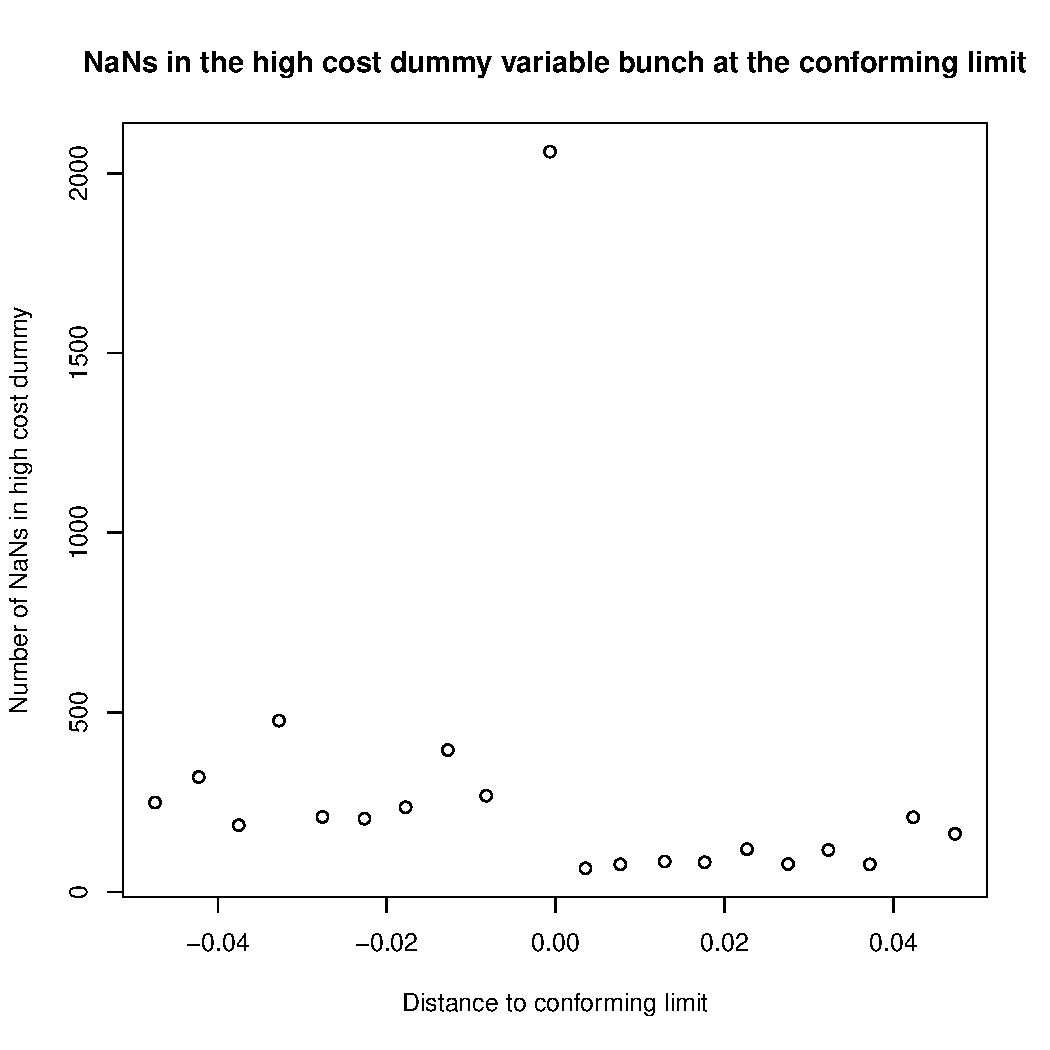
\includegraphics[scale=0.5]{figures/nans_in_high_cost_dummy_bunching.pdf}
    \end{center}
    
\end{figure}

\clearpage
\pagebreak

\begin{figure}

    \caption{LPW Table 7 --  NaNs in the High Cost County Dummy Variable Are Present in Multiple Counties}
    
    \begin{subfigure}{0.9\textwidth}
    \caption{Florida}
    \begin{center}
    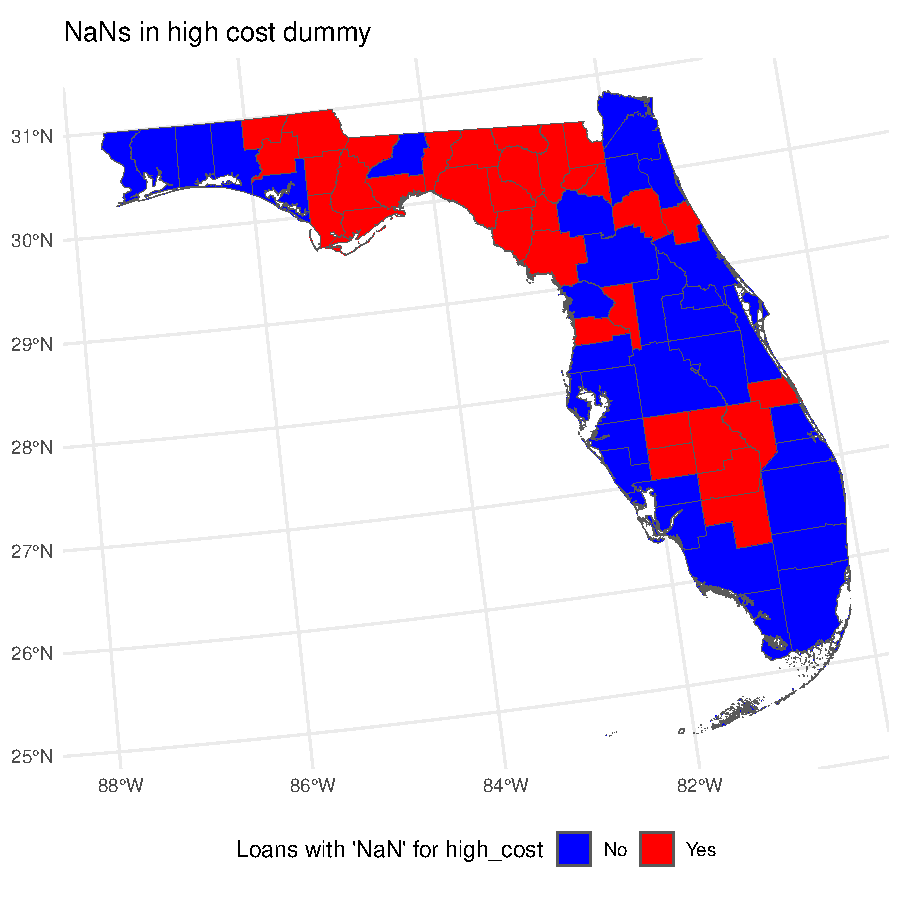
\includegraphics[scale=0.45]{figures/nans_in_high_cost_dummy_12.pdf}
    \end{center}
    \end{subfigure}

    \begin{subfigure}{0.9\textwidth}
        \caption{Louisiana}
        \begin{center}
        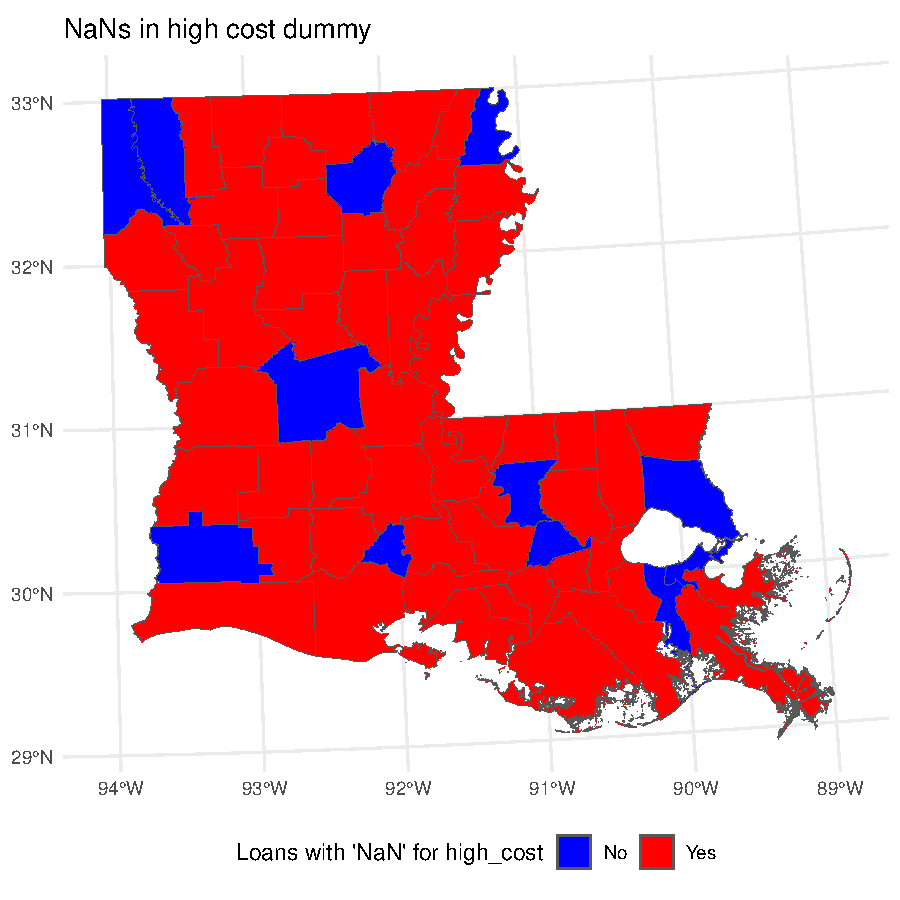
\includegraphics[scale=0.45]{figures/nans_in_high_cost_dummy_22.pdf}
        \end{center}
    \end{subfigure}

    \begin{subfigure}{0.9\textwidth}

        \caption{North Carolina}
        \begin{center}
            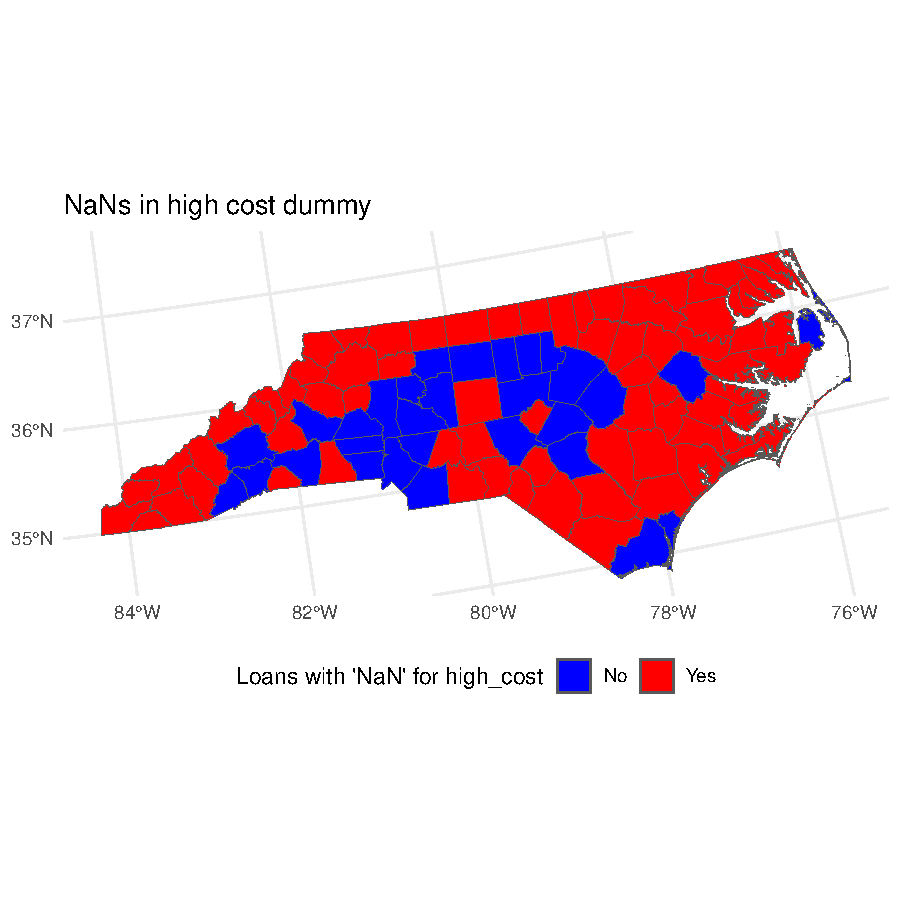
\includegraphics[scale=0.45]{figures/nans_in_high_cost_dummy_37.pdf}
            \end{center}
    \end{subfigure}
        
\end{figure}


\end{document}
